\documentclass[11pt, compress, t, notes = noshow, xcolor = table, 
aspectratio = 1610]{beamer}
\usepackage[]{graphicx}\usepackage[]{color}

\usepackage{framed}

\usepackage{alltt}
\newcommand{\SweaveOpts}[1]{}  % do not interfere with LaTeX
\newcommand{\SweaveInput}[1]{} % because they are not real TeX commands
\newcommand{\Sexpr}[1]{}       % will only be parsed by R

\usepackage[english]{babel}
\usepackage[utf8]{inputenc}
\usepackage{verbatim}
\usepackage{amsmath}
\usepackage{amsfonts}
\usepackage{bm}
\usepackage{csquotes}
\usepackage{multirow}
\usepackage{longtable}
\usepackage{enumerate}
\usepackage[absolute,overlay]{textpos}
\usepackage{algorithm}
\usepackage{algpseudocode}
\usepackage{eqnarray}
\usepackage{arydshln}
\usepackage{tabularx}
\usepackage{setspace}
\usepackage{colortbl}
\usepackage{mathtools}
\usepackage{wrapfig}
\usepackage{bm}
\usepackage{xcolor}
\usepackage{caption}
\captionsetup[figure]{font=tiny}
\usepackage[labelformat=empty]{caption}
\usepackage{subcaption}

% Defines macros and environments
% \usepackage{bbm}
% basic latex stuff
\newcommand{\pkg}[1]{{\fontseries{b}\selectfont #1}} %fontstyle for R packages
\newcommand{\lz}{\vspace{0.5cm}} %vertical space
\newcommand{\dlz}{\vspace{1cm}} %double vertical space
\newcommand{\oneliner}[1] % Oneliner for important statements
{\begin{block}{}\begin{center}\begin{Large}#1\end{Large}\end{center}\end{block}}


%new environments
\newenvironment{vbframe}  %frame with breaks and verbatim
{
 \begin{frame}[containsverbatim,allowframebreaks]
}
{
\end{frame}
}

\newenvironment{vframe}  %frame with verbatim without breaks (to avoid numbering one slided frames)
{
 \begin{frame}[containsverbatim]
}
{
\end{frame}
}

\newenvironment{blocki}[1]   % itemize block
{
 \begin{block}{#1}\begin{itemize}
}
{
\end{itemize}\end{block}
}

\newenvironment{fragileframe}[2]{  %fragile frame with framebreaks
\begin{frame}[allowframebreaks, fragile, environment = fragileframe]
\frametitle{#1}
#2}
{\end{frame}}


\newcommand{\myframe}[2]{  %short for frame with framebreaks
\begin{frame}[allowframebreaks]
\frametitle{#1}
#2
\end{frame}}

\newcommand{\remark}[1]{
  \textbf{Remark:} #1
}


\newenvironment{deleteframe}
{
\begingroup
\usebackgroundtemplate{
\includegraphics[width=\paperwidth,height=\paperheight]{../style/color/red.png}}
 \begin{frame}
}
{
\end{frame}
\endgroup
}
\newenvironment{simplifyframe}
{
\begingroup
\usebackgroundtemplate{
\includegraphics[width=\paperwidth,height=\paperheight]{../style/color/yellow.png}}
 \begin{frame}
}
{
\end{frame}
\endgroup
}\newenvironment{draftframe}
{
\begingroup
\usebackgroundtemplate{
\includegraphics[width=\paperwidth,height=\paperheight]{../style/color/green.jpg}}
 \begin{frame}
}
{
\end{frame}
\endgroup
}
% https://tex.stackexchange.com/a/261480: textcolor that works in mathmode
\makeatletter
\renewcommand*{\@textcolor}[3]{%
  \protect\leavevmode
  \begingroup
    \color#1{#2}#3%
  \endgroup
}
\makeatother

\usepackage{style/report}

% ------------------------------------------------------------------------------

\colorlet{highlightcol}{gray!90}
\newcommand{\maketag}[1]{\colorbox{highlightcol}{\textcolor{white}
{\MakeUppercase{#1}}}}
\newcommand{\highlight}[1]{\textcolor{highlightcol}{\textbf{#1}}}
\newcommand{\arritem}{\item[\highlight{$\rightarrow$}]}
\newcommand{\positem}{\item[$\highlight{+}$]}
\newcommand{\negitem}{\item[$\highlight{-}$]}
\newcommand{\flexitem}[1]{\item[$\highlight{#1}$]}
\newcommand{\conclbox}[1]{\fbox{\parbox{\textwidth}{\centering\textbf{#1}}}}
\colorlet{GRAY}{gray}

\let\code=\texttt
\let\proglang=\textsf

\setkeys{Gin}{width=0.9\textwidth}

% ------------------------------------------------------------------------------

\newcommand{\topo}{\mathcal{T}}
\newcommand{\mani}{\mathcal{M}}
\newcommand{\N}{\mathbb{N}}
\newcommand{\R}{\mathbb{R}}
\newcommand{\RD}{\mathbb{R}^D}
\newcommand{\Rd}{\mathbb{R}^d}
\newcommand{\setN}{\{1, 2, ..., N\}}
\newcommand{\X}{\mathcal{X}}
\newcommand{\x}{\bm{x}}
\newcommand{\Y}{\mathcal{Y}}
\newcommand{\y}{\bm{y}}
\newcommand{\pv}{\bm{p}}
\newcommand{\qv}{\bm{q}}
\newcommand{\W}{\bm{W}}
\newcommand{\M}{\bm{M}}
\newcommand{\Lap}{\bm{L}}
\newcommand{\D}{\bm{D}}
\newcommand{\K}{\bm{K}}
\newcommand{\G}{\bm{G}}
\newcommand{\I}{\bm{I}}
\newcommand{\E}{\bm{E}}
\newcommand{\twonorm}[1]{\left\lVert #1 \right\rVert^2}

% ------------------------------------------------------------------------------

\title{Semi-Supervised Locally Linear Embedding (SSLLE)}
\author{Lisa Wimmer}
\date{2021/26/02}

\setbeamertemplate{frametitle}{\expandafter\uppercase\expandafter
\insertframetitle}

\begin{document}

\lecturechapter{Application \& Sensitivity Analysis of Critical 
Hyperparameters}
\lecture{Semi-Supervised Locally Linear Embedding (SSLLE)}

% ------------------------------------------------------------------------------
% AGENDA
% ------------------------------------------------------------------------------

\LARGE
\begin{frame}{\textcolor{gray!90}{0 agenda}}
\normalsize
\vspace{-0.5cm}
\noindent \textcolor{gray!90}{\rule{\textwidth}{1pt}}
\smallskip

\begin{itemize}
\large
\flexitem{1} Problem
\flexitem{2} Local graph-based manifold learning (LGML)
\flexitem{3} Techniques
\begin{itemize}
  \large
  \flexitem{1} Unsupervised
  \flexitem{2} Semi-supervised ~ \maketag{SSLLE}
  \flexitem{3} Challenges
\end{itemize}
\flexitem{4} Sensitivity analysis
\begin{itemize}
  \large
  \flexitem{1} Setup
  \flexitem{2} Results
\end{itemize}
\flexitem{5} Discussion
\end{itemize}

\end{frame}

% ------------------------------------------------------------------------------
% MANIFOLD LEARNING PROBLEM
% ------------------------------------------------------------------------------

\LARGE
\begin{frame}{\textcolor{gray!90}{1 problem} ~~ manifold learning}
\normalsize
\vspace{-0.5cm}
\noindent \textcolor{gray!90}{\rule{\textwidth}{1pt}}
\smallskip

\textbf{Situation}. Rapidly increasing amount of data thanks to novel 
applications and data sources

\vspace{0.5cm}

\begin{minipage}[b]{0.7\textwidth}
  \raggedright
  \textbf{Problem.} High data dimensionality detrimental to
  \begin{itemize}
    \arritem Model functionality
    \arritem Interpretability
    \arritem Generalization ability
  \end{itemize}
  \medskip
  \textbf{Manifold assumption.} Data in high-dimensional observation
  space truly sampled from low-dimensional manifold
\end{minipage}%
\begin{minipage}[b]{0.3\textwidth}
  \begin{figure}[H]
    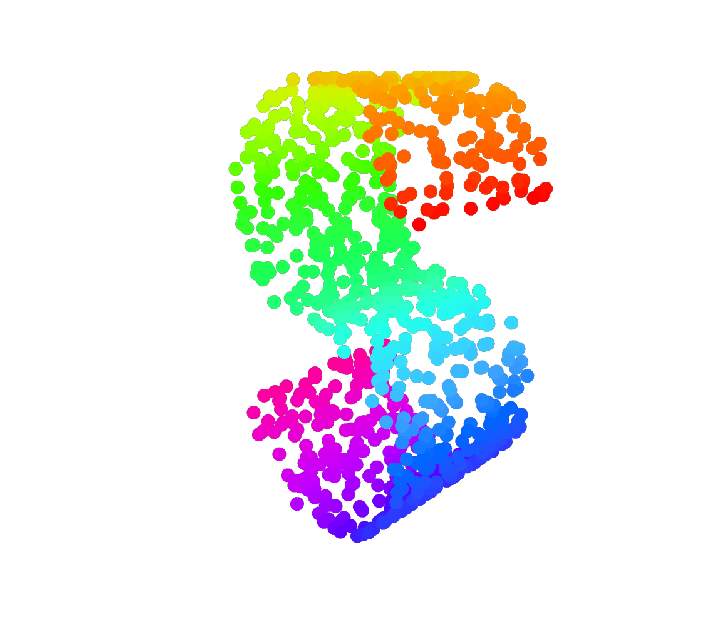
\includegraphics[trim = 70 30 70 30, clip, % left bottom right top
      width = 0.6\textwidth]{figures/s-curve}
  \end{figure}
\end{minipage}

\vfill

\conclbox{How to find a meaningful, structure-preserving embedding?}

\end{frame}

\LARGE
\begin{frame}{\textcolor{gray!90}{1 problem} ~~ manifold learning}
\normalsize
\vspace{-0.5cm}
\noindent \textcolor{gray!90}{\rule{\textwidth}{1pt}}
\smallskip

\textbf{Formal goal of manifold learning.}
\medskip
\begin{itemize}
  \arritem \textbf{Given.} Data $\X = (\x_1, \x_2, ..., \x_N)$, with $\x_i \in 
  \RD$ $\forall i \in \setN$ and $N, D \in \N$, supposedly lying on 
  $d$-dimensional manifold $\mani$ \\
  $\Rightarrow$ $\psi: \mani \rightarrow \Rd$ with $d \ll D, d \in \N$ \\
  $\Rightarrow$ $\X \sim \mani \subset \RD$ 
  \medskip
  \arritem \textbf{Goal.} Find $d$-dimensional Euclidean representation \\
  $\Rightarrow$ $\Y = (\y_1, \y_2, ..., \y_N)$, with 
  $\y_i = \psi(\x_i) \in \R^d$ $\forall i \in \setN$.
\end{itemize}

\vfill

\begin{figure}[H]
 \begin{subfigure}[c]{0.2\textwidth}
  \centering
   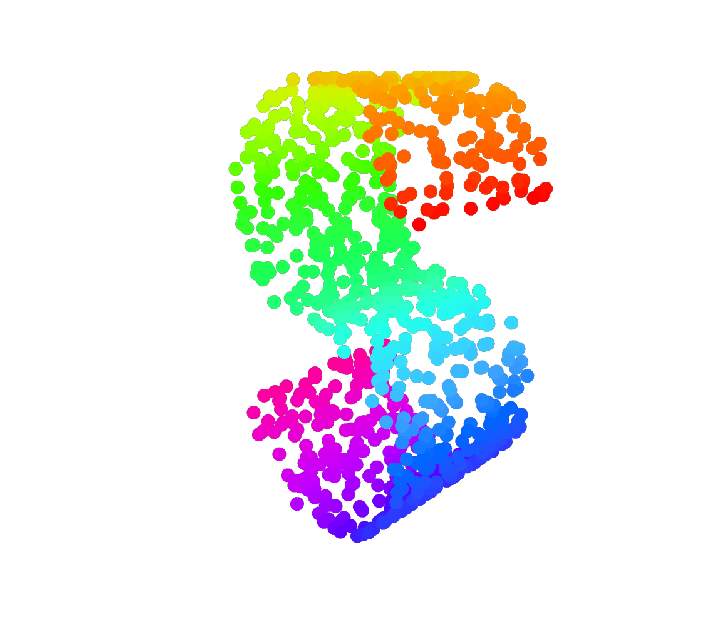
\includegraphics[trim = 70 30 70 30, clip, % left bottom right top
      width = 0.63\textwidth]{figures/s-curve}
 \end{subfigure}
 \hfill
 \begin{subfigure}[c]{0.7\textwidth}
   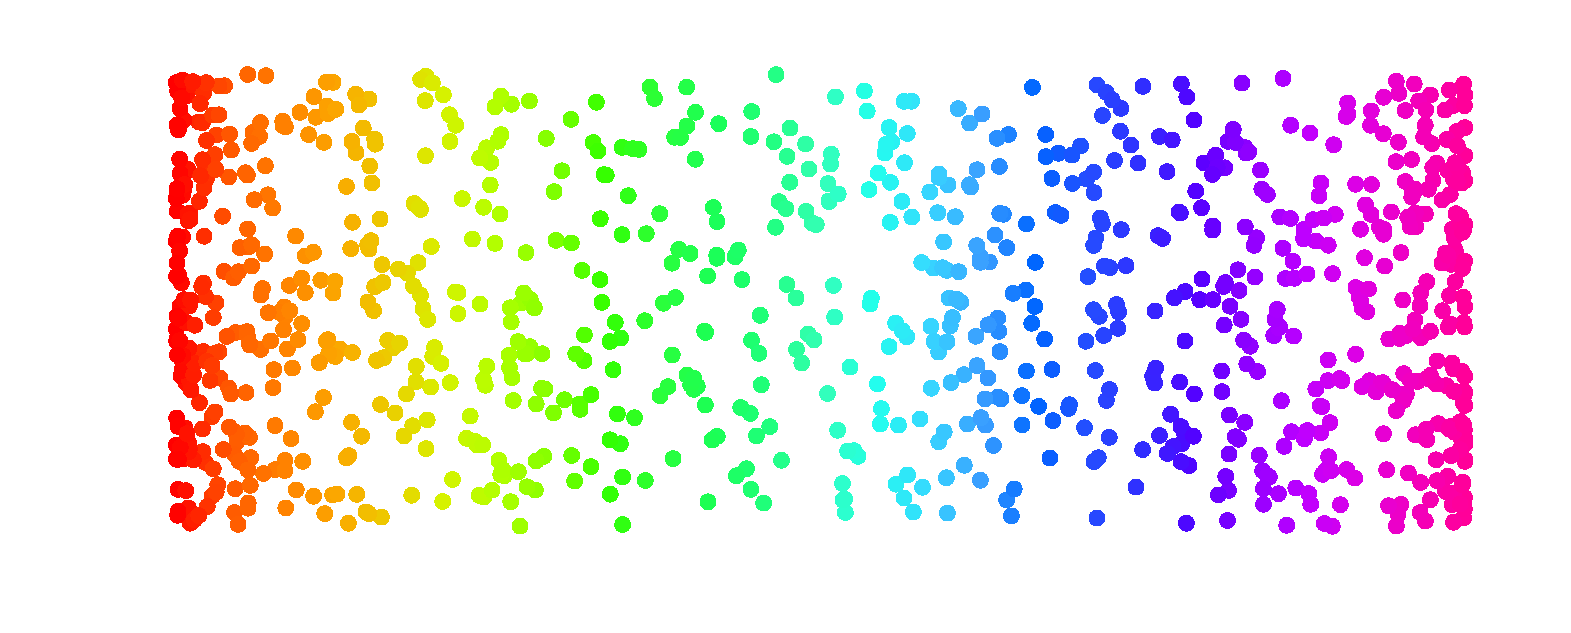
\includegraphics[trim = 80 20 0 0, clip, % left bottom right top
      width = 0.6\textwidth]{figures/s-curve-undone}
 \end{subfigure}
\end{figure}

\end{frame}

% ------------------------------------------------------------------------------
% LGML
% ------------------------------------------------------------------------------

\begin{frame}{}

\Huge
\hspace{0pt}
\vfill
\textbf{\highlight{2 ~~ LGML}}
\vfill
\hspace{0pt}

\end{frame}

% ------------------------------------------------------------------------------

\LARGE
\begin{frame}{\textcolor{gray!90}{2 lgml} ~~ taxonomy}
\normalsize
\vspace{-0.5cm}
\noindent \textcolor{gray!90}{\rule{\textwidth}{1pt}}
\smallskip

\textbf{Landscape}. Various approaches, many of which may be translated into one
another

\vspace{0.5cm}


\begin{minipage}[b]{0.65\textwidth}
  \begin{figure}[H]
    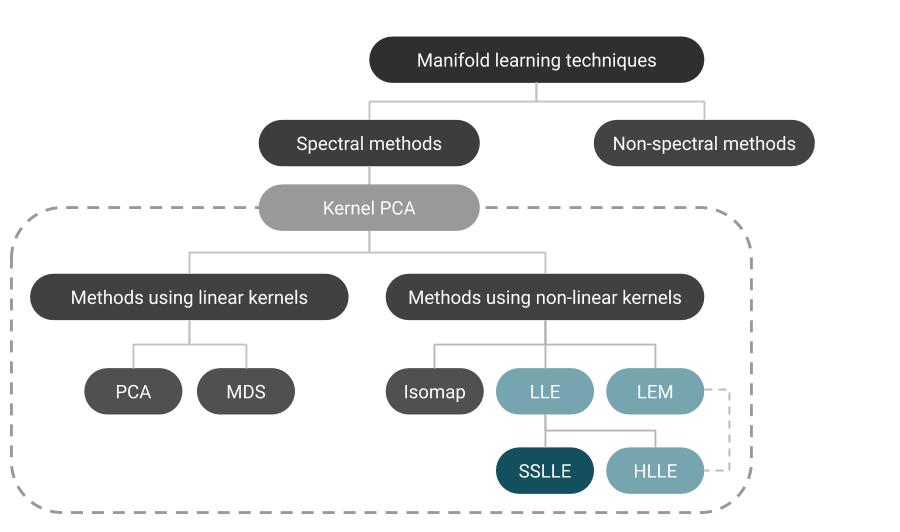
\includegraphics[trim = 0 20 25 0, clip, % left bottom right top
      width = \textwidth]{figures/models-overview}
  \end{figure}
\end{minipage}%
\begin{minipage}[b]{0.35\textwidth}
  \highlight{LEM} Laplacian eigenmaps \\
  \highlight{LLE} Locally linear embedding \\
  \highlight{HLLE} Hessian LLE \\
  \highlight{SSLLE} Semi-supervised LLE 
\end{minipage}

\end{frame}

% ------------------------------------------------------------------------------

\LARGE
\begin{frame}{\textcolor{gray!90}{2 lgml} ~~ concept}
\normalsize
\vspace{-0.5cm}
\noindent \textcolor{gray!90}{\rule{\textwidth}{1pt}}

% \footnotesize

\medskip

woteva

\end{frame}

% ------------------------------------------------------------------------------
% LGML TECHNIQUES
% ------------------------------------------------------------------------------

\begin{frame}{}

\Huge
\hspace{0pt}
\vfill
\textbf{\highlight{3 ~~ TECHNIQUES}}
\vfill
\hspace{0pt}

\end{frame}

% ------------------------------------------------------------------------------

\LARGE
\begin{frame}{\textcolor{gray!90}{3.1 unsupervised} ~~ lle}
\normalsize
\vspace{-0.5cm}
\noindent \textcolor{gray!90}{\rule{\textwidth}{1pt}}

% \footnotesize

\medskip

woteva

\end{frame}

% ------------------------------------------------------------------------------

\LARGE
\begin{frame}{\textcolor{gray!90}{3.2 semi-supervised} ~~ sslle}
\normalsize
\vspace{-0.5cm}
\noindent \textcolor{gray!90}{\rule{\textwidth}{1pt}}

% \footnotesize

\medskip

woteva

\end{frame}

% ------------------------------------------------------------------------------

\LARGE
\begin{frame}{\textcolor{gray!90}{3.3 challenges} ~~ neighborhood relations}
\normalsize
\vspace{-0.5cm}
\noindent \textcolor{gray!90}{\rule{\textwidth}{1pt}}

% \footnotesize

\medskip

woteva

\end{frame}

% ------------------------------------------------------------------------------
% SENSITIVITY ANALYSIS
% ------------------------------------------------------------------------------

\begin{frame}{}

\Huge
\hspace{0pt}
\vfill
\textbf{\highlight{4 ~~ SENSITIVITY ANALYSIS}}
\vfill
\hspace{0pt}

\end{frame}

% ------------------------------------------------------------------------------

\LARGE
\begin{frame}{\textcolor{gray!90}{4.1 setup} ~~ scenarios}
\normalsize
\vspace{-0.5cm}
\noindent \textcolor{gray!90}{\rule{\textwidth}{1pt}}

% \footnotesize

\medskip

woteva

\end{frame}

% ------------------------------------------------------------------------------

\LARGE
\begin{frame}{\textcolor{gray!90}{4.1 setup} ~~ evaluation}
\normalsize
\vspace{-0.5cm}
\noindent \textcolor{gray!90}{\rule{\textwidth}{1pt}}

% \footnotesize

\medskip

woteva

\end{frame}

% ------------------------------------------------------------------------------

\LARGE
\begin{frame}{\textcolor{gray!90}{4.2 results} ~~ foo}
\normalsize
\vspace{-0.5cm}
\noindent \textcolor{gray!90}{\rule{\textwidth}{1pt}}

% \footnotesize

\medskip

woteva

\end{frame}

% ------------------------------------------------------------------------------
% DISCUSSION
% ------------------------------------------------------------------------------

\begin{frame}{}

\Huge
\hspace{0pt}
\vfill
\textbf{\highlight{5 ~~ DISCUSSION}}
\vfill
\hspace{0pt}

\end{frame}

% ------------------------------------------------------------------------------

\LARGE
\begin{frame}{\textcolor{gray!90}{5 discussion} ~~ foo}
\normalsize
\vspace{-0.5cm}
\noindent \textcolor{gray!90}{\rule{\textwidth}{1pt}}

% \footnotesize

\medskip

woteva

\end{frame}

% ------------------------------------------------------------------------------
% BIBLIOGRAPHY
% ------------------------------------------------------------------------------

\begin{frame}{}

\Huge
\hspace{0pt}
\vfill
\textbf{\highlight{REFERENCES}}
\vfill
\hspace{0pt}

\end{frame}

% ------------------------------------------------------------------------------

\begin{frame}{}
\normalsize

G. Randauthor (2021): Most Relevant Shit, THE Journal, frontpage (what else)

\end{frame}

% ------------------------------------------------------------------------------

\endlecture

\end{document}